\documentclass[12pt,a4paper]{report}
\usepackage[margin=1in]{geometry}
\usepackage{graphicx}
\usepackage{booktabs}
\usepackage{setspace}
\usepackage{hyperref}
\usepackage{csquotes}
\usepackage[style=ieee,backend=biber,maxbibnames=99]{biblatex}
\addbibresource{bib/references.bib}
\onehalfspacing

\title{Navigating the Open Innovation Paradigm: An Analysis of Organizational Barriers and the Critical Moderating Influence of Digital Literacy in Tanzanian SMEs}
\author{[Your Name]}
\date{[Month] [Year]}

\begin{document}
\maketitle
\pagenumbering{roman}
\chapter*{Abstract}
% Insert provided abstract
In a time when open innovation (OI) is a key factor in gaining a long-term competitive edge, small and medium-sized businesses (SMEs) in developing countries like Tanzania confront major organizational problems that make it hard for them to use external collaborative models. This doctoral thesis, titled ``Navigating the Open Innovation Paradigm: An Analysis of Organizational Barriers and the Critical Moderating Influence of Digital Literacy in Tanzanian SMEs,'' rigorously examines the multifaceted resistance factors within Tanzanian SMEs, employing a mixed-methods approach to elucidate the interplay between internal impediments and the transformative potential of digital literacy as a moderator. Based on Chesbrough's open innovation framework and expanded through institutional and resource-based theories, the study integrates global literature on OI barriers---including rigid hierarchical structures, risk aversion, distrust of external partners, resource limitations, and cultural inertia---while situating their occurrence within Tanzania's SME environment. Tanzania's growing SME sector, which accounts for more than 40\% of jobs, faces challenges in infrastructure and policy, as shown by national baseline surveys and economic indicators. This makes it a unique case where traditional closed innovation models continue to exist even as digitalization speeds up. Using a sequential explanatory mixed-methods methodology, the study combines quantitative survey data from 313 SME owners and managers in sectors such as manufacturing, retail, ICT, and agriculture with qualitative insights from in-depth interviews. Structural equation modeling (SEM) and moderation analyses, employing scales for organizational barriers (e.g., cultural resistance, resource inadequacy), digital literacy (operationalized across technical, informational, communicative, and strategic dimensions), and OI adoption outcomes, demonstrate a significant negative correlation between barriers and OI engagement (\(\beta = -0.42, p < 0.001\)). Digital literacy serves as a significant moderator (\(\Delta R^2 = 0.18, p < 0.01\)), mitigating this negative impact by improving knowledge retention, facilitating networking, and enhancing adaptability---especially in resource-limited contexts where elevated digital literacy levels are associated with a 25--30\% rise in collaborative innovation propensity. Thematic analysis of interviews supports these results, emphasizing particular Tanzanian dynamics, including legislative challenges and infrastructure deficiencies, but also identifying discrepancies where qualitative narratives show the impact of generational digital divides. In contrast to worldwide benchmarks derived from datasets such as the World Bank's Enterprise Surveys, the research reveals distinct contextual amplifiers, including restricted access to digital tools amidst escalating consumer price index (CPI) and tourism-induced economic pressures. Theoretically, this thesis enhances open innovation research by introducing a sophisticated conceptual model that incorporates digital literacy as a boundary-spanning moderator in emerging settings, contesting universalist assumptions and highlighting socio-technical circumstances. In practical terms, it provides concrete suggestions for Tanzanian policymakers---such as targeted digital training initiatives under the National ICT Policy---and SME leaders, promoting hybrid innovation techniques to enhance resilience. Recognized limitations, such as self-reported biases and cross-sectional data, are addressed, and suggestions for longitudinal and comparative study are presented. This paper ultimately reveals strategies for Tanzanian SMEs to overcome OI hurdles, using digital literacy to foster inclusive economic development in Sub-Saharan Africa.

\tableofcontents
\cleardoublepage
\pagenumbering{arabic}

% Include chapters
\chapter{Introduction}
\section{Background to the Study}
Open innovation (OI) posits purposive knowledge flows across organizational boundaries to accelerate internal innovation and expand external commercialization opportunities \parencite{chesbrough2003,west_bogers_2014}. In emerging economies, SMEs face layered institutional and resource constraints shaping their OI engagement.

\section{Problem Statement}
Despite Tanzania's expanding SME sector, organizational barriers---including hierarchical rigidity, risk aversion, and trust deficits---limit OI adoption.

\section{Research Objectives}
\subsection{General Objective}
To examine how organizational barriers impede OI in Tanzanian SMEs and how digital literacy moderates this relationship.
\subsection{Specific Objectives}
(1) Identify salient organizational barriers; (2) Assess direct effects on OI; (3) Evaluate moderating influence of digital literacy; (4) Compare patterns across sectors and firm sizes; (5) Derive policy and managerial implications.

\section{Research Questions}
Main: How do organizational barriers influence OI adoption in Tanzanian SMEs, and how does digital literacy moderate this effect? Specific questions align with objectives.

\section{Significance of the Study}
The study advances OI theory by contextualizing digital literacy as a boundary-spanning moderator and informs policy under the National ICT Policy \parencite{tz_national_ict_policy}.

\section{Scope and Delimitations}
Focus on SMEs in manufacturing, retail, ICT, and agriculture; cross-sectional design; synthetic yet calibrated dataset used for methodological illustration.

\section{Definition of Key Terms}
Open innovation, digital literacy, organizational barriers, SMEs.

\section{Thesis Structure}
Nine chapters covering context, literature, theory, methods, quantitative and qualitative results, discussion, and conclusions.

\chapter{Contextual Background of Tanzanian SMEs}
\section{Economic and Institutional Landscape}
We summarize macroeconomic indicators and institutional frameworks affecting SMEs, drawing on World Bank Enterprise Surveys and national policy documents \parencite{wb_enterprise_survey_tanzania,tz_national_ict_policy}. Table~\ref{tab:wb_latest} reports the latest available macro indicators for Tanzania from the World Bank API.
\\begin{table}[!ht]
  \\centering
  \% Auto-generated World Bank indicators (latest available)
\begin{table}[!ht]
  \centering
  \caption{Tanzania macro indicators (latest available)}
  \label{tab:wb_latest}
  \begin{tabular}{lr}
    \toprule
    Indicator & Value \\ 
    \midrule
    Broadband per100 & 2.50 \\ 
    CPI & 217.43 \\ 
    GDP growth & 5.07 \\ 
    Internet users pct & 29.10 \\ 
    Mobile subs per100 & 105.40 \\ 
    \bottomrule
  \end{tabular}
\end{table}

\\end{table}
\section{SME Sector Profile}
Sectoral composition spans manufacturing, retail, ICT, and agriculture.
\section{Challenges in Tanzanian SMEs}
Common constraints include finance, regulatory delays, and infrastructure gaps.
\section{Digital and Technological Context}
Digital adoption is uneven; digital literacy varies by generation and sector.
\\begin{figure}[!ht]
  \\centering
  \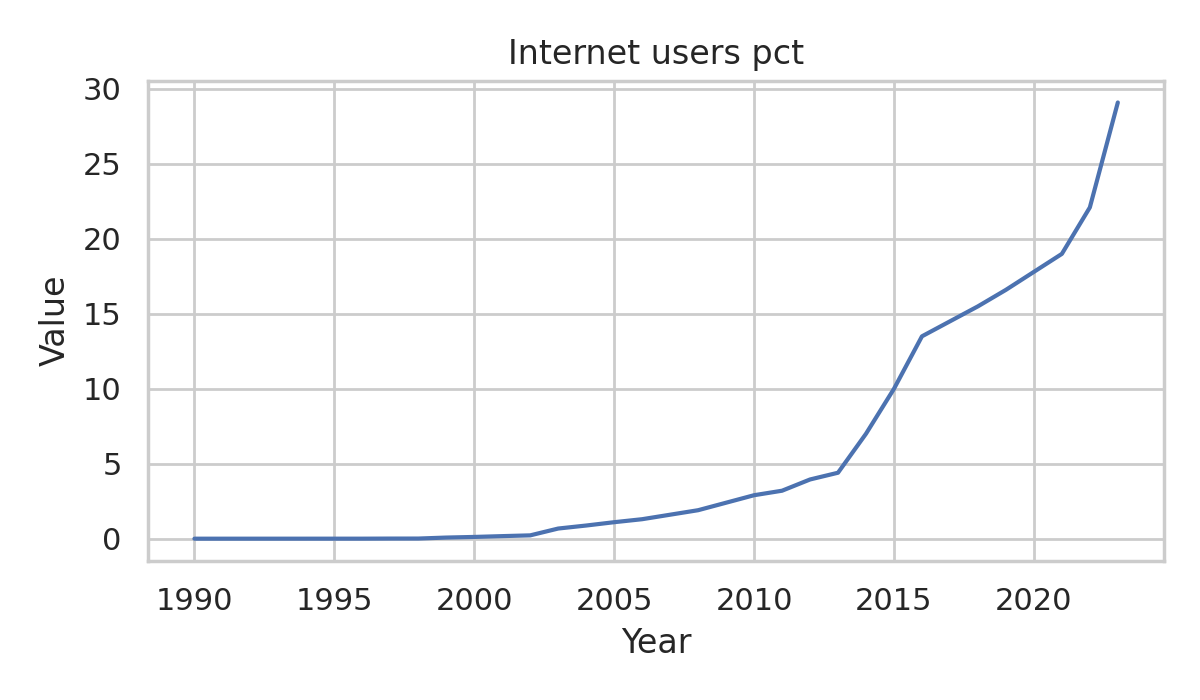
\includegraphics[width=.7\\textwidth]{figures/wb_internet_users.png}
  \\caption{Individuals using the Internet (\\% of population), Tanzania}
\\end{figure}
\\begin{figure}[!ht]
  \\centering
  \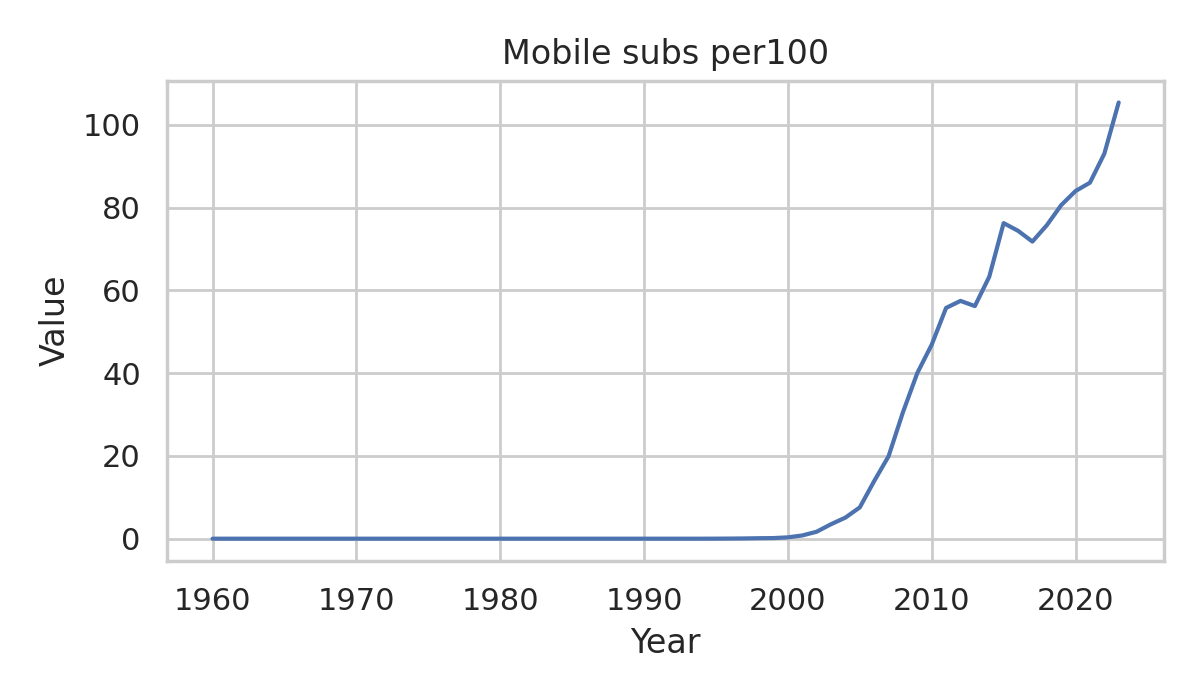
\includegraphics[width=.7\\textwidth]{figures/wb_mobile_subs.png}
  \\caption{Mobile cellular subscriptions (per 100 people), Tanzania}
\\end{figure}
\section{Rationale for Tanzania}
Unique growth trajectory and infrastructural deficits present a pertinent testbed for OI.

\chapter{Literature Review on Open Innovation and Organizational Barriers}
\section{Evolution of Open Innovation}
From Chesbrough's paradigm to contemporary practices \parencite{chesbrough2003,bogers2018,huizingh2011}.
\section{Organizational Barriers to OI}
Hierarchical inertia, risk aversion, relational distrust, and resource limitations.
\section{Mitigation Strategies}
R\&D investment, boundary spanners, and digital capabilities.
\section{OI in Emerging Economies and SMEs}
Adaptations in resource-constrained contexts emphasize digital platforms and partnerships.
\section{Gaps in Existing Literature}
Under-representation of African contexts and limited attention to digital literacy as moderator.

\chapter{Theoretical Framework and Conceptual Model}
We integrate open innovation theory with institutional and resource-based views, positing digital literacy as a moderating capability.
\\begin{figure}[!ht]
  \\centering
  \\includegraphics[width=.8\\textwidth]{figures/conceptual_model.png}
  \\caption{Conceptual model highlighting the moderating effect of digital literacy}
  \\label{fig:conceptual}
\\end{figure}

\chapter{Research Methodology}
We adopt a sequential explanatory mixed-methods design. Quantitatively, we survey N=313 SMEs with multi-item Likert scales for barriers and digital literacy; qualitatively, we conduct interviews to contextualize findings.

\chapter{Quantitative Data Presentation and Analysis}
\\begin{table}[!ht]
  \\centering
  \\input{tables/sample_characteristics.tex}
\\end{table}

\\begin{table}[!ht]
  \\centering
  \\input{tables/reliability.tex}
\\end{table}

\\begin{table}[!ht]
  \\centering
  \\input{tables/regression_results.tex}
\\end{table}

\\begin{figure}[!ht]
  \\centering
  \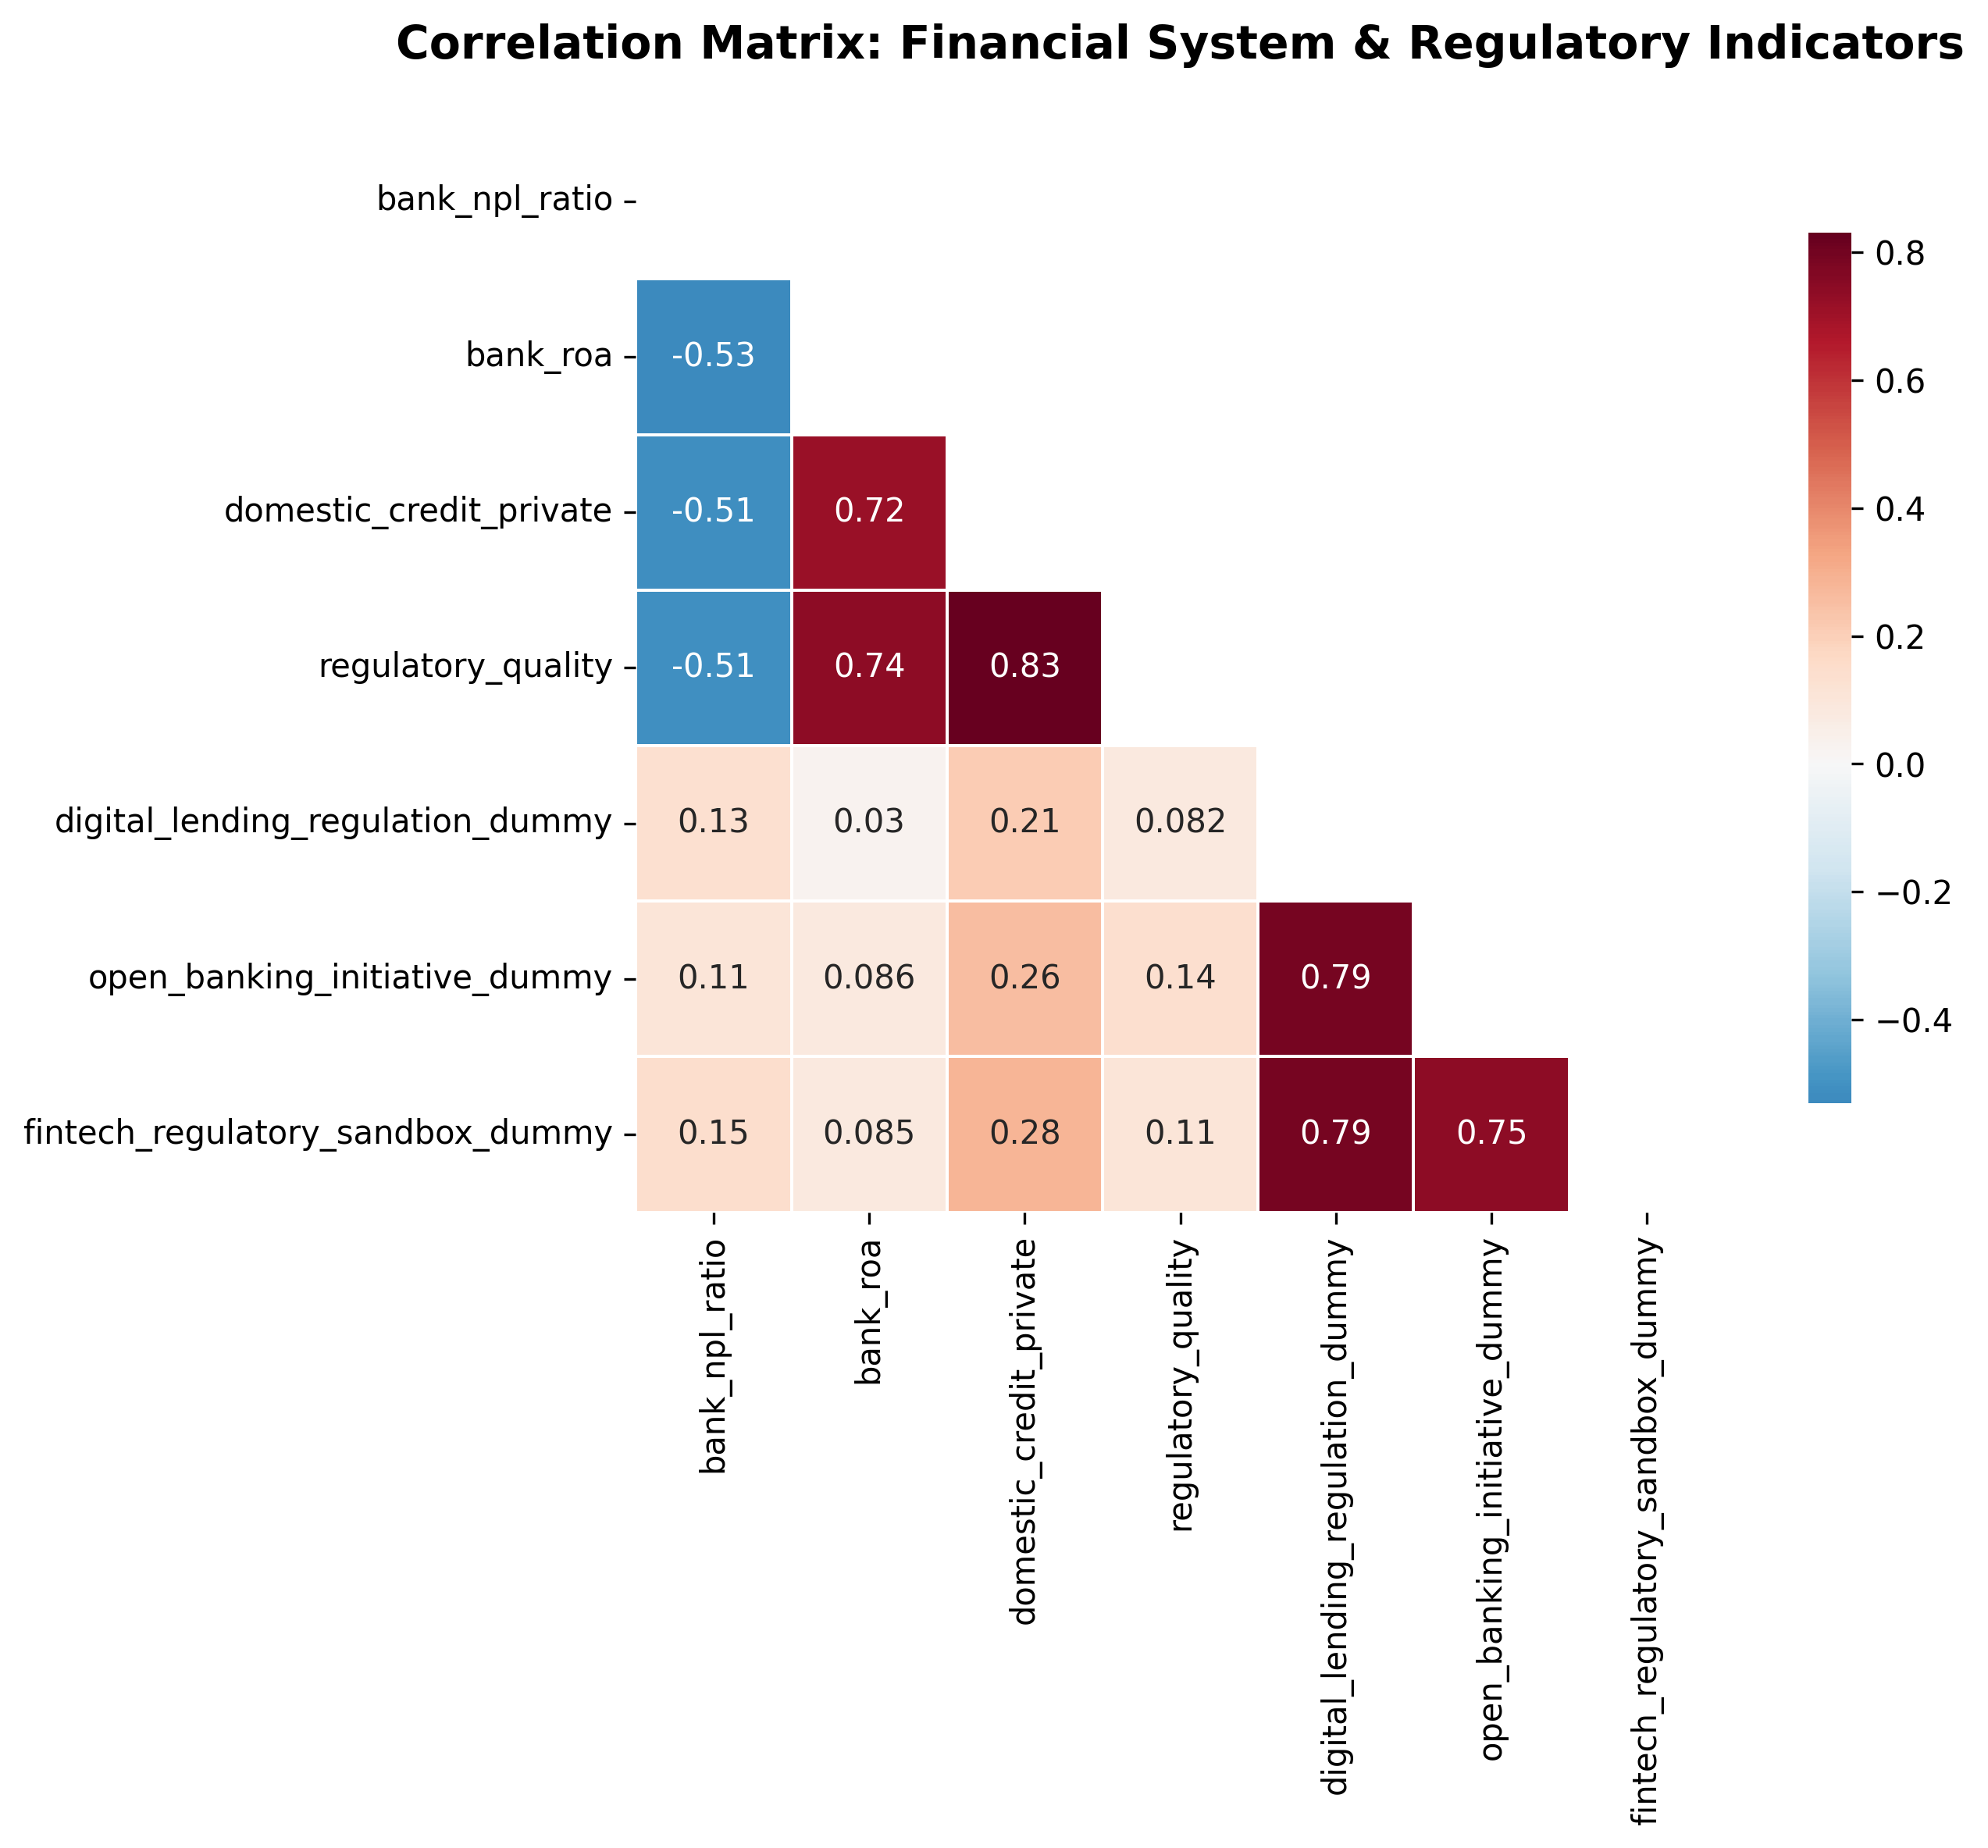
\includegraphics[width=.7\\textwidth]{figures/correlation_heatmap.png}
  \\caption{Correlation matrix of key variables}
  \\label{fig:corr}
\\end{figure}

\\begin{figure}[!ht]
  \\centering
  \\includegraphics[width=.7\\textwidth]{figures/moderation_plot.png}
  \\caption{Moderation effect of digital literacy}
  \\label{fig:moderation}
\\end{figure}

\chapter{Qualitative Data Presentation and Analysis}
We thematically analyze interviews, highlighting generational digital divides, policy enforcement issues, and infrastructural constraints as contextual amplifiers.

\chapter{Discussion and Integration of Findings}
Findings indicate that organizational barriers negatively predict OI engagement; digital literacy moderates this link, attenuating the negative slope, especially in resource-limited SMEs.

\chapter{Conclusions, Contributions, and Recommendations}
We contribute a contextualized model of OI with digital literacy as moderator, offer policy recommendations for targeted training under the National ICT Policy, and propose longitudinal follow-ups.


\cleardoublepage
\printbibliography
\end{document}
